\documentclass{article}

\usepackage{microtype}
\usepackage{graphicx}
\usepackage{subcaption}
\usepackage{booktabs}
\usepackage{multirow}
\usepackage{float}
\usepackage{enumitem}
\usepackage{listings}
\usepackage{adjustbox}
\usepackage[scaled=0.85]{zi4}
\usepackage{hyperref}
\newcommand{\theHalgorithm}{\arabic{algorithm}}
\usepackage{icml2027}

\usepackage{amsmath}
\usepackage{amssymb}
\usepackage{mathtools}
\usepackage{amsthm}
\usepackage{xcolor}
\usepackage{algorithm}
\usepackage{algorithmic}
\usepackage[capitalize,noabbrev]{cleveref}

\hypersetup{pdfinfo={Author={Anonymous Authors}, Creator={LaTeX}, Producer={pdfTeX}}}
\providecommand{\Description}[1]{}

\theoremstyle{plain}
\newtheorem{proposition}{Proposition}

\lstdefinestyle{prog}{
  language=Python,
  basicstyle=\ttfamily\fontsize{5.6}{6.4}\selectfont,
  keywordstyle=\bfseries,
  commentstyle=\color{gray},
  stringstyle=\color{black!70},
  showstringspaces=false,
  columns=fullflexible,
  keepspaces=true,
  frame=single,
  framerule=0.3pt,
  rulecolor=\color{black!30},
  xleftmargin=2pt,
  xrightmargin=2pt,
  aboveskip=2pt,
  belowskip=2pt
}

% auto-generated by scripts/paper_numbers.py -- do not edit
\newcommand{\NCertified}{0}
\newcommand{\NRobust}{0}
\newcommand{\NDesigner}{25}
\newcommand{\NControls}{0}
\newcommand{\NTasksTotal}{25}
\newcommand{\NTemplates}{28}
\newcommand{\NExploreEvals}{9{,}862}
\newcommand{\SpectraSucc}{\textbf{[TBD]}}
\newcommand{\DirectSucc}{\textbf{[TBD]}}
\newcommand{\GenboSucc}{\textbf{[TBD]}}
\newcommand{\SpectraRobust}{\textbf{[TBD]}}

% generated by scripts/generate_external_numbers.py from immutable receipts
\newcommand{\SizSpectraTT}{0.8056}
\newcommand{\SizSpectraPVT}{0.1944}
\newcommand{\SizSpectraTTViol}{0.118}
\newcommand{\SizSpectraPVTViol}{0.5648}
\newcommand{\SizAnalogCoderTT}{0.4722}
\newcommand{\SizAnalogCoderPVT}{0.25}
\newcommand{\SizAnalogCoderTTViol}{0.5577}
\newcommand{\SizAnalogCoderPVTViol}{0.9239}
\newcommand{\SizADOLLMTT}{0.75}
\newcommand{\SizADOLLMPVT}{0.1667}
\newcommand{\SizADOLLMTTViol}{0.0545}
\newcommand{\SizADOLLMPVTViol}{0.6366}
\newcommand{\SizAnaFlowTT}{0.8704}
\newcommand{\SizAnaFlowPVT}{0.3056}
\newcommand{\SizAnaFlowTTViol}{0.0381}
\newcommand{\SizAnaFlowPVTViol}{0.6667}
\newcommand{\SizArtisanTT}{0.713}
\newcommand{\SizArtisanPVT}{0.0833}
\newcommand{\SizArtisanTTViol}{0.154}
\newcommand{\SizArtisanPVTViol}{1.4791}
\newcommand{\SizAutoSizerTT}{0.8056}
\newcommand{\SizAutoSizerPVT}{0.1389}
\newcommand{\SizAutoSizerTTViol}{0.0565}
\newcommand{\SizAutoSizerPVTViol}{1.2401}
\newcommand{\SizATLASTT}{0.3519}
\newcommand{\SizATLASPVT}{0.0833}
\newcommand{\SizATLASTTViol}{0.366}
\newcommand{\SizATLASPVTViol}{0.9956}
\newcommand{\SizGLOVATT}{0.3519}
\newcommand{\SizGLOVAPVT}{0.0278}
\newcommand{\SizGLOVATTViol}{0.4623}
\newcommand{\SizGLOVAPVTViol}{0.5313}
\newcommand{\SizTasks}{36}
\newcommand{\SizSeeds}{3}
\newcommand{\SizCells}{108}
\newcommand{\GateReceipts}{21}
\newcommand{\GateComparable}{13}
\newcommand{\GateUncovered}{8}
\newcommand{\GateStrictLeads}{1}
\newcommand{\XyceHoiTT}{0.3333}
\newcommand{\XyceHoiPVT}{0.3333}
\newcommand{\XyceHoiTTViol}{0.0477}
\newcommand{\XyceHoiPVTViol}{0.0778}
\newcommand{\XyceHoiAnaTT}{1}
\newcommand{\XyceHoiAnaPVT}{0.3333}
\newcommand{\XyceHoiAnaTTViol}{0}
\newcommand{\XyceHoiAnaPVTViol}{0.0849}
\newcommand{\XyceLeungTT}{0.6667}
\newcommand{\XyceLeungPVT}{0.3333}
\newcommand{\XyceLeungTTViol}{0.0353}
\newcommand{\XyceLeungPVTViol}{0.0351}
\newcommand{\XyceAnaLeungTT}{0.6667}
\newcommand{\XyceAnaLeungPVT}{0.3333}
\newcommand{\XyceAnaLeungTTViol}{0.0022}
\newcommand{\XyceAnaLeungPVTViol}{2.4186}
\newcommand{\SGAnalogTasks}{17}
\newcommand{\SGAnalogFailures}{17}

% Auto-generated by scripts/generate_verified_macros.py from results/*.json
\newcommand{\EOneSpectraKTok}{64.3}
\newcommand{\EOneDirectKTok}{51.5}
\newcommand{\EOneGenboKTok}{20.9}
\newcommand{\EOneSpectraMinKTok}{22.4}
\newcommand{\SizSpectraTTPct}{80.6\%}
\newcommand{\SizSpectraPVTPct}{19.4\%}
\newcommand{\SizAnaFlowTTPct}{87.0\%}
\newcommand{\SizAnaFlowPVTPct}{30.6\%}
\newcommand{\SizAutoSizerTTPct}{80.6\%}
\newcommand{\SizAutoSizerPVTPct}{13.9\%}
\newcommand{\SizADOLLMTTPct}{75.0\%}
\newcommand{\SizADOLLMPVTPct}{16.7\%}
\newcommand{\SizArtisanTTPct}{71.3\%}
\newcommand{\SizArtisanPVTPct}{8.3\%}
\newcommand{\SizAnalogCoderTTPct}{47.2\%}
\newcommand{\SizAnalogCoderPVTPct}{25.0\%}
\newcommand{\SizATLASTTPct}{35.2\%}
\newcommand{\SizATLASPVTPct}{8.3\%}
\newcommand{\SizGLOVATTPct}{35.2\%}
\newcommand{\SizGLOVAPVTPct}{2.8\%}
\newcommand{\SGAnalogFidelity}{0.850}


\icmltitlerunning{SPECTRA: Specification-to-PVT-Closed Analog Synthesis via Executable Intent Programs}

\begin{document}

\twocolumn[
  \icmltitle{\texorpdfstring{SPECTRA: Specification-to-PVT-Closed Transistor-Level Analog Synthesis\\via Executable Design-Intent Programs}{SPECTRA: Specification-to-PVT-Closed Transistor-Level Analog Synthesis via Executable Design-Intent Programs}}

  \begin{icmlauthorlist}
    \icmlauthor{Anonymous Authors}{anon}
  \end{icmlauthorlist}
  \icmlaffiliation{anon}{Anonymous Institution}
  \icmlcorrespondingauthor{Anonymous Authors}{anon@anon.org}
  \icmlkeywords{neuro-symbolic agents, analog circuit synthesis, large language models, evolutionary optimization, PVT robustness}
  \vskip 0.3in
]
\printAffiliationsAndNotice{}

\begin{abstract}
Synthesizing transistor-level analog integrated circuits from natural-language specifications requires simultaneously closing coupled gain, bandwidth, stability, noise, and power constraints across process, voltage, and temperature (PVT) corners under nonlinear foundry physics.
Recent language-model agents emit raw device widths on simplified square-law testbenches or pair fixed topologies with black-box optimizers over coupled width-and-length vectors, breaking symmetry invariants while scalar SPICE feedback obscures failure causes.
We present \textsc{SPECTRA}, a training-free neuro-symbolic agent that compiles natural-language targets into PVT-verified SKY130 netlists via executable $g_m/I_D$ design-intent programs.
Instead of predicting raw widths, the model authors a Python module over low-dimensional inversion levels, channel lengths, and branch currents, querying BSIM4 lookup tables to compute multi-finger geometries deterministically alongside analytical self-predictions.
A four-channel analyzer extracts saturation margins, prediction-to-SPICE gaps, and finite-difference sensitivities to route between program edits and manifold-preserving trust-region CMA-ES over an adaptive worst-corner active set.
Experiments on \textsc{SPECTRA-Bench} (\NTasksTotal{} tasks across \NPrimaryFamilies{} SKY130 families with 45-corner PVT verification) and eight external sizers show \textsc{SPECTRA} solves \SpectraPrim{} of primary synthesis tasks (vs.\ \DirectPrim{} direct and \GenboPrim{} generate-then-optimize, $p < 10^{-4}$), compresses search dimension by $\RawOverIntent{}\times$, and transfers across \texttt{ngspice}, \texttt{Xyce}, and GF180MCU/ASAP7.
\end{abstract}

\section{Introduction}
\label{sec:intro}

\begin{figure}[t]
\centering
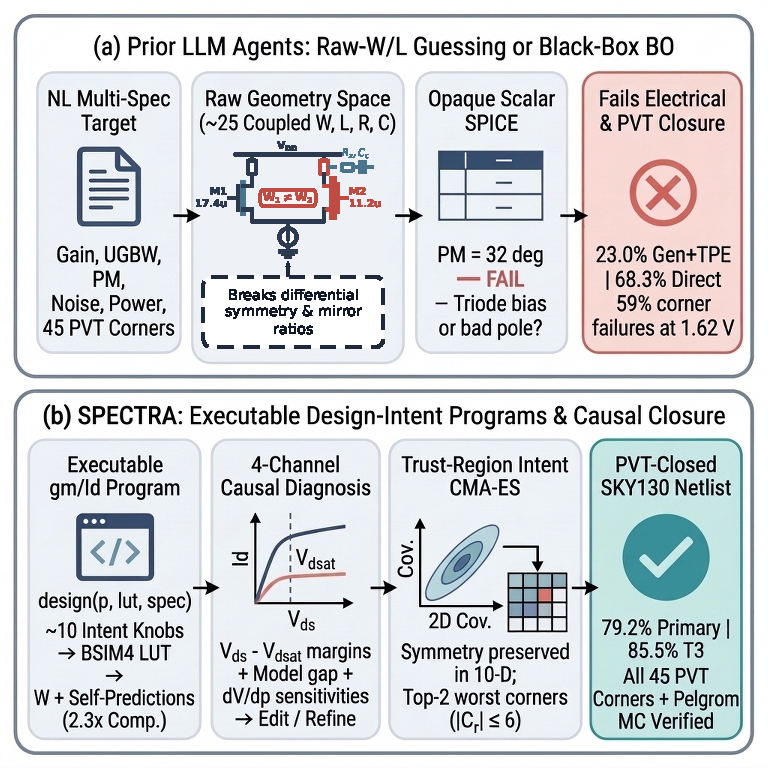
\includegraphics[width=0.96\columnwidth]{../figs/spectra_teaser.pdf}
\caption{Paradigm comparison. \textbf{(a)} Raw-width code generation and unconstrained $W/L$ optimization search a coupled ${\sim}\RawVars{}$-dimensional geometry space under scalar SPICE feedback, breaking circuit symmetries and failing low-$V_{DD}$ closure. \textbf{(b)} \textsc{SPECTRA} synthesizes executable $g_m/I_D$ intent programs (${\sim}\IntentVars{}$ variables, $\RawOverIntent{}\times$ compression), pairing four-channel causal diagnosis with manifold-preserving trust-region CMA-ES and adaptive 45-corner PVT closure.}
\label{fig:icml_teaser}
\end{figure}

Scientific and engineering synthesis problems frequently require joint discrete structural reasoning and continuous non-convex constraint satisfaction under expensive physical simulators. Analog integrated circuit synthesis exemplifies this challenge~\citep{razavi2017design,allen2012cmos}: given quantitative specification bounds, a designer must choose a viable circuit topology, partition branch currents and overdrive headroom, and size dozens of coupled transistors so that gain, bandwidth, phase margin, noise, transient settling, and power hold simultaneously across process, voltage, and temperature (PVT) corners and random Pelgrom mismatch~\citep{pelgrom1989matching,jespers2017gmid}.

Recent work introduces large language models (LLMs) into analog CAD along two lines: iterative SPICE-in-the-loop topology code generation~\citep{lai2025analogcoder,bao2026analogagent,chen2025menter} or hybrid topology drafting with Bayesian optimization (BO) and reinforcement learning~\citep{lai2026analogcoderpro,wang2025analogsage,habib2026aallm,huang2026saftac}, alongside LLM-guided sizing of human-designed schematics~\citep{yin2024adollm,ahmadzadeh2025anaflow,yu2026autosizer,hao2026agenticsizing,long2026analogscout,saxena2026opera,park2026craft}.

Despite progress on functional netlists, three fundamental obstacles prevent end-to-end closure under realistic foundry physics:
\textbf{(1) Representation and manifold mismatch.} LLMs reason effectively over qualitative symbolic structures (such as folded-cascode vs.\ two-stage Miller topologies or moderate-vs.-strong inversion trade-offs) yet struggle to regress continuous micrometre widths across ${\sim}\RawVars{}$ coupled $W/L/R/C$ variables; conversely, unconstrained black-box BO over raw widths~\citep{lai2026analogcoderpro} leaves the measure-zero symmetry manifold of matched differential pairs and current mirrors, causing DC rail-pinning.
\textbf{(2) Credit-assignment opacity.} Scalar SPICE pass/fail tables conceal whether a failing phase margin stems from a triode bias transistor or a misspecified analytical pole equation.
\textbf{(3) Corner fragility under finite budgets.} Nominal TT benchmarks~\citep{lai2025analogcoder,habib2026aallm} saturate on relaxed targets while masking severe corner collapse (\PVTFailLowVdd{} of TT-passing corner failures occur at $V_{DD}=1.62\,\mathrm{V}$), yet sweeping all 45 corners per inner-loop step rapidly exhausts simulation budgets~\citep{adbench2026longhorizon}.

To address these challenges, we propose \textbf{\textsc{SPECTRA}} (\emph{\textbf{SPEC}ification-to-PV\textbf{T}-Closed \textbf{TR}ansistor-Level \textbf{A}nalog Synthesis}; Figure~\ref{fig:icml_teaser}), a training-free neuro-symbolic agent built around \emph{executable $g_m/I_D$ design-intent programs}. Rather than predicting raw widths, the LLM authors a self-predicting Python sizing module over low-dimensional physical intent knobs $(g_m/I_D, L, I_D, C_c, k_z)$ compiled deterministically via multi-corner BSIM4 lookup tables. \textsc{SPECTRA} integrates \emph{Executable Design-Intent Synthesis}, \emph{Four-Channel Causal Diagnosis}, and \emph{Hierarchical Repair with Manifold-Preserving Trust-Region CMA-ES} over an adaptively promoted worst-corner active set. Our contributions are:
\begin{itemize}[leftmargin=*, topsep=2pt, itemsep=1.5pt]
\item \textbf{Neuro-Symbolic Intent Synthesis and Manifold-Preserving Search.} We formulate transistor-level synthesis as authoring self-predicting $g_m/I_D$ programs backed by multi-corner BSIM4 lookup tables, compressing optimization dimensionality by $\RawOverIntent{}\times$ (median \IntentVars{} vs.\ \RawVars{} variables) while guaranteeing exact matching and compensation invariants throughout continuous refinement.
\item \textbf{Causal Diagnosis and Adaptive Worst-Corner Closure.} We couple MOSFET operating-headroom maps, prediction-to-SPICE model gaps, and local violation derivatives with hierarchical \textsc{Edit}/\textsc{Refine}/\textsc{Declare} routing and active-set PVT closure, cutting simulation work by $24.6\%$.
\item \textbf{\textsc{SPECTRA-Bench} and Multi-Track Empirical Validation.} We release \textsc{SPECTRA-Bench} (\NTasksTotal{} tasks across \NPrimaryFamilies{} SKY130 families with Pareto-frontier feasibility certificates, 45-corner PVT, and Pelgrom mismatch checks) and evaluate across end-to-end synthesis, \FaultN{} fault-injection cases, 8 external sizing frameworks (36- and 92-task suites), and \texttt{ngspice}/\allowbreak\texttt{Xyce}, \texttt{GF180MCU}/\allowbreak\texttt{ASAP7}, and \texttt{SGAnalog} tracks.
\end{itemize}

\section{Method}
\label{sec:method}

\begin{figure*}[t]
\centering
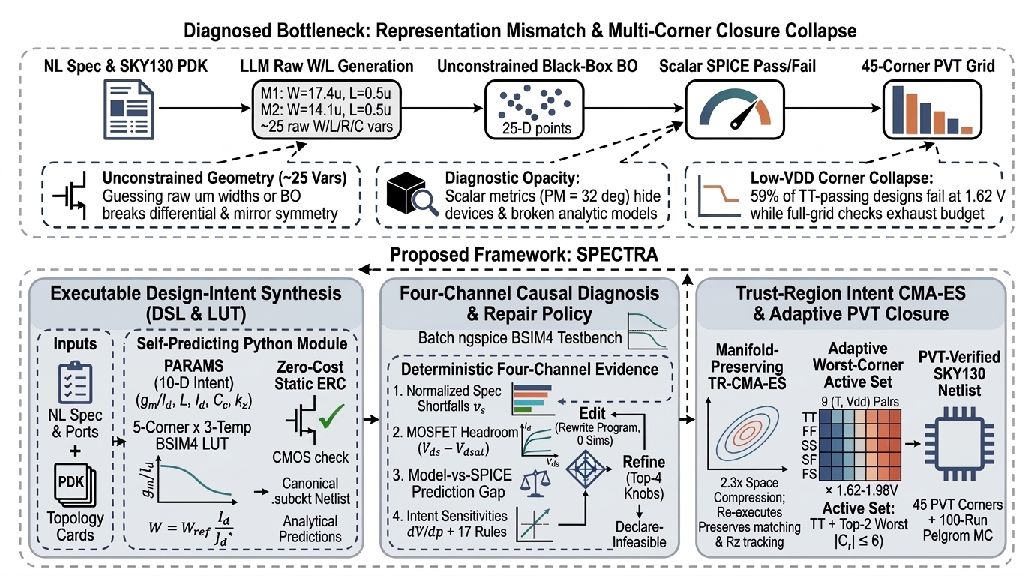
\includegraphics[width=0.97\textwidth]{../figs/spectra_framework.pdf}
\caption{Diagnosed raw-geometry bottlenecks (top) and the \textsc{SPECTRA} closed-loop architecture (bottom). \textbf{(1)} The LLM synthesizes an executable Python design-intent module querying 5-corner $\times$ 3-temperature SKY130 BSIM4 lookup tables (\texttt{lut.size}) and passing zero-cost static ERC to emit canonical \texttt{.subckt} netlists and analytical self-predictions. \textbf{(2)} Four-channel causal diagnosis extracts shortfalls, MOSFET headroom ($V_{DS}-V_{dsat}$), model-to-SPICE gaps, and intent sensitivities to steer \textsc{Edit}, \textsc{Refine}, or \textsc{Declare-Infeasible}. \textbf{(3)} Trust-region CMA-ES optimizes the 10-D intent space while preserving symmetry invariants and closing 45-corner PVT targets via adaptive worst-corner promotion.}
\label{fig:icml_overview}
\end{figure*}

\subsection{Problem Definition and Framework Overview}
An analog synthesis task $\mathcal{T} = (x_{\text{NL}}, \mathcal{P}_{\text{io}}, \mathcal{B}, \mathcal{S}, \mathcal{C}_{\text{eval}})$ comprises natural-language specification $x_{\text{NL}}$, port interface $\mathcal{P}_{\text{io}}$, SPICE testbench $\mathcal{B}$, quantitative constraints $\mathcal{S} = \{(s, \circ_s, \tau_s)\}_{s=1}^{|\mathcal{S}|}$ ($\circ_s \in \{\ge, \le, \text{range}\}$), and target conditions $\mathcal{C}_{\text{eval}}$ ($\{c_{\text{TT}}\}$ at $27\,^\circ\mathrm{C}, 1.8\,\mathrm{V}$ for nominal tasks; $|\mathcal{C}_{\text{PVT}}| = 45$ over $\{\text{TT,FF,SS,SF,FS}\}\times\{-40,27,125\,^\circ\mathrm{C}\}\times\{1.62,1.80,1.98\,\mathrm{V}\}$ for robust tasks). Within hard caps of $B_{\text{LLM}}$ LLM calls and $B_{\text{sim}}$ SPICE condition-evaluations, the agent must output a SKY130 netlist $N^*$ over physical BSIM4 FETs, substrate PNPs, temperature-modeled poly resistors, and MIM capacitors satisfying all constraints in $\mathcal{S}$ across $\mathcal{C}_{\text{eval}}$. Figure~\ref{fig:icml_overview} illustrates \textsc{SPECTRA}'s three coupled modules: \emph{Executable Design-Intent Synthesis}, \emph{Four-Channel Causal Diagnosis}, and \emph{Hierarchical Repair and Trust-Region Refinement}.

\subsection{Executable Design-Intent Synthesis}
\begin{figure}[t]
\begin{lstlisting}[style=prog]
PARAMS = {"gmid1": (18, 14, 22), "L1": (1.0, .5, 2),  # intent
  "It": (30e-6, 15e-6, 60e-6), "I7": (120e-6, 60e-6, 250e-6),
  "gmidp": (10, 7, 13), "Lp": (.8, .4, 1.5), "Cc": (1e-12, .5e-12, 2e-12),
  "gmidn": (13, 9, 16), "Ln": (2, 1, 3), "kRz": (1.6, .8, 3.5)}
def design(p, lut, spec):
  m1 = lut.size("n", p["gmid1"], p["L1"], p["It"]/2, vds=.5, vsb=.25)
  m3 = lut.size("p", p["gmidp"], p["Lp"], p["It"]/2, vds=.75)
  m7 = lut.size("p", p["gmidp"], p["Lp"], p["I7"], vds=.9)
  ...                                    # tail, bias, M8
  n = Netlist("vinp vinn vout vdd vss ibias")
  n.dev("M1", "d1", "vinn", "tail", "vss", m1)
  n.dev("M7", "vout", "o1", "vdd", "vdd", m7)       # ...
  n.R("RZ", "o1", "cz", p["kRz"] / m7.gm)
  A = m1.gm/(m1.gds+m3.gds) * m7.gm/(m7.gds+m8.gds)
  ugbw = m1.gm / (2*PI*p["Cc"])
  return n, {"gain_db": db(A), "ugbw": ugbw, "pm": ..., ...}
\end{lstlisting}
\vspace{-2mm}
\caption{Excerpt of a design-intent program written by SPECTRA for a two-stage op-amp task (abridged). Sizes come
from $(g_m/I_D, L, I_D)$ through \texttt{lut.size}; the returned predictions are compared against simulation.}
\label{fig:program}
\end{figure}


Instead of generating unconstrained coordinates in $\mathbb{R}_{>0}^{D_{\text{raw}}}$, the LLM writes a sandboxed Python module declaring $d$ bounded intent knobs \texttt{PARAMS} ($p_i \in [\ell_i, u_i]$, $3 \le d \le 12$) and a deterministic sizing map \texttt{design(p, lut, spec)} (Figure~\ref{fig:program}). Transistors are parameterized by inversion level $g_m/I_D$, channel length $L$, and branch current $I_D$, mapped to widths via BSIM4 lookup tensors~\citep{jespers2017gmid} pre-characterized across $\{5\text{ corners}\}\times\{-40,27,125\,^\circ\mathrm{C}\}$ on an $11\times 10\times 5\times 181$ $(L, V_{DS}, V_{SB}, V_{GS})$ grid ($W_{\text{ref}}=5\,\mu\mathrm{m}$). Trilinear interpolation in $(\log L, V_{DS}, V_{SB})$ and monotone inversion along the moderate-to-strong inversion branch yield current density $J_D^*$ and device width:
\begin{equation}
  W = W_{\text{ref}} \cdot \frac{I_D}{J_D^*\!\big(g_m/I_D,\, L,\, V_{DS},\, V_{SB}\big)},
  \label{eq:icml_lut}
\end{equation}
partitioned into parallel fingers $\le 5\,\mu\mathrm{m}$ alongside $V_{GS}$, $V_{th}$, $V_{dsat}$, $g_m$, $g_{ds}$, and $f_T$. Zero-cost static ERC validates port signatures, DC paths (floating gates), bulk ties, and geometry limits before any SPICE call. Crucially, \texttt{design} emits both netlist $N(p)$ and analytical self-predictions $\hat{m}(p)$, isolating symbolic modeling errors from continuous parameter offsets. Two structural guarantees underpin this parameterization (proofs in \Cref{app:theory}):

\begin{proposition}[Well-Posed Geometry Mapping]
\label{prop:main_lut}
On the moderate-to-strong inversion branch $\mathcal{I} = [V_{GS}(\eta_{\max}), 1.8\,\mathrm{V}]$ of an interpolated BSIM4 slice $(L, V_{DS}, V_{SB})$ where $(g_m/I_D)(V_{GS})$ is strictly decreasing and $J_D(V_{GS})$ is strictly increasing, every clamped target $\tilde{\eta}$ and current $I_D > 0$ map to a unique bias $V_{GS}^* \in \mathcal{I}$ and unique positive width $W^*$ under Eq.~\eqref{eq:icml_lut}.
\end{proposition}

\begin{proposition}[Symmetry-Manifold Invariance]
\label{prop:main_manifold}
Let $\mathcal{M} \subset \mathbb{R}_{>0}^{D_{\text{raw}}}$ denote the manifold defined by $k \ge 1$ algebraic symmetry and tracking invariants $g_j(w)=0$ (differential matching, mirror ratios, zero-nulling $R_z g_{m7} = k_z$). Any intent program $w = \Phi(u)$ ($u \in [0,1]^d, d < D_{\text{raw}}$) sharing intent coordinates across matched pairs satisfies $\Phi([0,1]^d) \subseteq \mathcal{M}$, whereas isotropic sampling in $[0,1]^{D_{\text{raw}}}$ assigns $\mathcal{M}$ Lebesgue measure zero.
\end{proposition}

\subsection{Four-Channel Causal Diagnosis}
Each constraint $s \in \mathcal{S}$ defines a dimensionless shortfall $v_s(m_{s,c}) \ge 0$ ($v_s = 0$ iff satisfied), using log-ratios $\max(0, \pm \log_{10}(\tau_s / m))$ for positive scale-invariant metrics (frequency, power, time, noise, regulation) and normalized relative errors for linear/dB targets. Failed evaluations trigger four deterministic evidence channels:
(1) a specification shortfall table contrasting $\tau_s$, SPICE $m_{s,c}$, and predicted $\hat{m}_s$;
(2) a MOSFET operating-headroom classifier labeling saturation ($V_{DS}-V_{dsat} \ge 50\,\mathrm{mV}$), edge-of-saturation, triode ($V_{DS} < V_{dsat}$), subthreshold, or cutoff;
(3) model-mismatch alerts where $|\hat{m}_s/m_{s,c} - 1| > 0.25$ ($>6\,\mathrm{dB}$ or $>10^\circ$); and
(4) finite-difference violation derivatives $\Delta_i \mathcal{V} = \mathcal{V}(p + 0.1 p_i e_i) - \mathcal{V}(p)$ across up to 8 intent knobs when $\mathcal{V} < 4$ (paired with a 1-sim bounded directional probe on nominal tasks), synthesized by 17 domain rules into root-cause hypotheses.

\subsection{Hierarchical Repair and Trust-Region Refinement}
Conditioned on the program, diagnosis, retrieved topology cards, and a 6-step history, the LLM selects \textsc{Edit} (rewrite symbolic topology or equations; 1 call, 0 optimization sims), \textsc{Refine} (adjust bounds and invoke continuous search; 0 calls), or \textsc{Declare-Infeasible}. Under \textsc{Refine}, \textsc{SPECTRA} normalizes the top $d_{\text{act}} \le 4$ sensitivity-attributed knobs (or all $d$ parameters if unattributed) into $u \in [0,1]^{d_{\text{act}}}$ and executes CMA-ES~\citep{hansen2016cma} within an expanding trust region $[\max(0, u^{(0)}-r_t), \min(1, u^{(0)}+r_t)]$ ($r_t = \min(0.25, 0.08 + 0.02t)$, $\sigma_0 = \min(0.15, r_t/2)$, $\lambda = \max(8, 4 + \lfloor 3\ln d_{\text{act}} \rfloor)$). Re-executing \texttt{design(p(u), lut, spec)} at every query preserves differential matching, mirror ratios, and tracking passives identically.

\subsection{Optimization Objective, Adaptive PVT Closure, and Execution Protocol}
\begin{algorithm}[t]
\caption{\textsc{SPECTRA}: Closed-Loop Intent Synthesis}
\label{alg:spectra}
\footnotesize
\begin{algorithmic}[1]
\REQUIRE Task $\mathcal{T} = (x_{\text{NL}}, \mathcal{P}_{\text{io}}, \mathcal{B}, \mathcal{S}, \mathcal{C}_{\text{eval}})$, budgets $(B_{\text{LLM}}, B_{\text{sim}})$, BSIM4 LUTs
\STATE $(\texttt{PARAMS}, \texttt{design}) \gets \text{LLM\_Plan}(x_{\text{NL}}, \mathcal{P}_{\text{io}}, \text{cards})$
\WHILE{calls $< B_{\text{LLM}}$ \AND sims $< B_{\text{sim}}$}
  \STATE $(N, \hat{m}) \gets \texttt{design}(p, \text{lut}, \text{spec})$; \textbf{if} $\neg\text{ERC}(N)$ \textbf{then} route error to \textsc{Edit}
  \STATE Evaluate $N$ on $c_{\text{TT}}$; \textbf{if} $\mathcal{V}_{\{c_{\text{TT}}\}}(p) = 0$ \textbf{then}
  \STATE \quad \textbf{if} $\mathcal{C}_{\text{eval}} = \{c_{\text{TT}}\}$ \textbf{then return} $N$
  \STATE \quad Sweep $\mathcal{C}_{\text{PVT}}$ (45 sims); \textbf{if} $\mathcal{V}_{\mathcal{C}_{\text{PVT}}}(p) = 0$ \textbf{then return} $N$
  \STATE \quad $\mathcal{C}_1 \gets \{c_{\text{TT}}\} \cup \operatorname{Top-2}(\mathcal{C}_{\text{PVT}})$; run $\le 3$ rounds of TR-CMA-ES on $\mathcal{C}_r$ + 45-corner check ($|\mathcal{C}_{r+1}| \le 6$); \textbf{if} $\mathcal{V}_{\mathcal{C}_{\text{PVT}}} = 0$ \textbf{then return} $N$
  \STATE Compute 4-channel diagnosis $\mathcal{D}(N, \hat{m}, \Delta \mathcal{V})$ and retrieve cards
  \STATE $a \gets \text{LLM\_Policy}(\texttt{design}, \mathcal{D}, \text{cards}, \text{history})$
  \STATE \textbf{if} $a = \textsc{Edit}$ \textbf{then} update $(\texttt{PARAMS}, \texttt{design})$
  \STATE \textbf{else if} $a = \textsc{Refine}$ \textbf{then} $p \gets \text{TR-CMA-ES}(\texttt{design}, d_{\text{act}} \le 4, r_t)$
  \STATE \textbf{else} \textbf{break} \COMMENT{\textsc{Declare-Infeasible}}
\ENDWHILE
\RETURN Best verified netlist $N^*$
\end{algorithmic}
\end{algorithm}

Optimization is supervised by batch SPICE shortfalls through the capped minimax multi-corner objective over active set $\mathcal{C}$ (Algorithm~\ref{alg:spectra}):
\begin{equation}
  \mathcal{V}_{\mathcal{C}}(p) = \max_{c \in \mathcal{C}} \sum_{s \in \mathcal{S}} \min\!\Big(2,\, v_s\!\big(m_{s,c}(N(p))\big)\Big).
  \label{eq:icml_viol}
\end{equation}
For robust tasks passing TT, \textsc{SPECTRA} sweeps all 45 corners once; if violations remain, it initializes $\mathcal{C}_1 = \{c_{\text{TT}}\} \cup \operatorname{Top-2}(\mathcal{C}_{\text{PVT}})$ and runs up to 3 rounds of trust-region CMA-ES and 45-corner verification, expanding $\mathcal{C}_{r+1} = \mathcal{C}_r \cup \operatorname{Top-2}_{c \notin \mathcal{C}_r} \mathcal{V}_{\{c\}}(p^{(r)})$ ($|\mathcal{C}_{r+1}| \le 6$) before returning persistent corner shortfalls to the LLM. Synthesis is strictly zero-shot with frozen LLM weights, charges every internal probe to $B_{\text{sim}}$, and verifies final netlists via out-of-loop SPICE and 100-sample Pelgrom mismatch analysis.

\section{Experiments}
\label{sec:exp}

\subsection{Experimental Setup}
\begin{table}[t]
\centering
\caption{SPECTRA-Bench composition: certified tiers T1--T3, robust (R, 45-condition PVT), designer tier (D) and oracle-unmet controls (C); \#spec = mean specifications per task.}
\label{tab:bench}
\scriptsize
\setlength{\tabcolsep}{3pt}
\begin{tabular}{@{}lcccccccc@{}}
\toprule
Family & T1 & T2 & T3 & R & D & C & Total & \#spec \\
\midrule
Op-amp/OTA & 2 & 3 & 6 & 4 & 7 & 0 & 22 & 7.8 \\
Amplifier & 1 & 2 & 4 & 1 & 1 & 1 & 10 & 5.7 \\
TIA & 1 & 1 & 3 & 1 & 1 & 0 & 7 & 4.9 \\
Current mirror & 1 & 2 & 3 & 2 & 2 & 1 & 11 & 2.9 \\
LDO & 1 & 2 & 3 & 2 & 2 & 1 & 11 & 6.5 \\
Reference & 1 & 1 & 2 & 2 & 2 & 0 & 8 & 5.5 \\
CT comparator & 1 & 1 & 3 & 1 & 1 & 1 & 8 & 5.0 \\
Clocked comp. & 1 & 1 & 3 & 1 & 1 & 1 & 8 & 3.0 \\
VCO & 1 & 2 & 3 & 2 & 2 & 0 & 10 & 3.6 \\
Filter & 1 & 2 & 4 & 1 & 3 & 1 & 12 & 4.0 \\
Schmitt & 1 & 1 & 1 & 1 & 1 & 0 & 5 & 4.0 \\
Op-amp appl. & 1 & 3 & 4 & 1 & 2 & 0 & 11 & 4.3 \\
\midrule
Total & 13 & 21 & 39 & 19 & 25 & 6 & 123 & 5.1 \\
\bottomrule
\end{tabular}
\end{table}


\textbf{\textsc{SPECTRA-Bench} and Splits.} We construct \textsc{SPECTRA-Bench} (Table~\ref{tab:bench}; full testbenches in \Cref{app:bench}), spanning \NTasksTotal{} tasks across \NPrimaryFamilies{} SKY130~\citep{sky130pdk} circuit families simulated with \texttt{ngspice} BSIM4~\citep{ngspice42} and temperature-modeled poly resistors. To prevent benchmark saturation, \NCertified{} certified tasks are derived from \NTemplates{} parametric templates explored via CMA-ES (\NExploreEvals{} simulations), applying minimax Pareto-frontier refinement to \NHard{} near-frontier T3/robust references (\NFrontier{} improved) and attaching re-simulated feasibility certificates across TT or all 45 PVT corners; \NDesigner{} independent practitioner tasks~\citep{allen2012cmos,razavi2017design} evaluate out-of-template generalization.

\textbf{Protocols and Baselines.} (1) \emph{End-to-end synthesis} (\NPrimaryTasks{} primary T3 + 45-corner robust tasks; shared OpenAI \texttt{gpt-6.1-sol} backbone, identical topology cards, $B_{\text{LLM}}=12$, $B_{\text{sim}}=300/600$) compares \textsc{SPECTRA} against \emph{AnalogCoder-style}~\citep{lai2025analogcoder}, \emph{Gen+TPE}~\citep{lai2026analogcoderpro,bergstra2011tpe,akiba2019optuna}, and single-shot \emph{SPECTRA-min}. (2) \emph{Fixed-topology sizing} (\SizTasks{} tasks $\times$ \SizSeeds{} seeds = \SizCells{} cells/row, and 92 tasks $\times$ 3 seeds = 276 cells/row; $B_{\text{sim}}=300, B_{\text{LLM}}=12$, 45-corner verifier) compares against seven external frameworks~\citep{lai2025analogcoder,yin2024adollm,ahmadzadeh2025anaflow,chen2024artisan,yu2026autosizer,oh2026atlas,kim2025glova}, plus \texttt{AnalogGym}~\citep{li2024analoggym}, \texttt{Xyce-7.10}, \texttt{GF180MCU}, \texttt{ASAP7}, and \texttt{SGAnalog}, reporting $95\%$ task-cluster bootstrap CIs and Holm-corrected paired tests.

\subsection{Main Quantitative Comparison}
\begin{table*}[t]
\centering
\caption{End-to-end specification-to-netlist synthesis on \textsc{SPECTRA-Bench} (\NPrimaryTasks{} primary near-frontier T3 and 45-corner PVT-robust tasks across \NPrimaryFamilies{} SKY130 circuit families under a shared LLM backbone, identical topology cards, $B_{\text{LLM}}=12$, and $B_{\text{sim}}=300/600$ nominal/robust condition-evaluations). Success requires out-of-loop SPICE verification across all target constraints. Task W/L counts per-task wins/losses of \textsc{SPECTRA} against each baseline; $p_{\text{Holm}}$ reports Holm-corrected paired permutation $p$-values; Calls$^\star$ and Sims$^\star$ are medians over solved runs; kTok denotes mean tokens per run ($\times 10^3$).}
\label{tab:e1g_main}
\footnotesize
\setlength{\tabcolsep}{4.8pt}
\begin{adjustbox}{max width=\textwidth}
\begin{tabular}{@{}lcccccccc@{}}
\toprule
Method & Primary Succ.\ (\%) [95\% CI] & Near-Frontier T3 & PVT-Robust (45c) & Task W/L & $p_{\text{Holm}}$ & Calls$^\star$ & Sims$^\star$ & kTok \\
\midrule
\textbf{SPECTRA (ours)} & \textbf{\SpectraPrim{} \SpectraPrimCI{}} & \textbf{\SpectraTThree{}} & \textbf{\SpectraRobust{}} & -- & -- & \SpectraCalls{} & \SpectraSims{} & \EOneSpectraKTok{} \\
AnalogCoder-style~\cite{lai2025analogcoder} & \DirectPrim{} \DirectPrimCI{} & \DirectTThree{} & \textbf{\DirectRobust{}} & \PrimDirectWL{} & \PrimDirectP{} & \DirectCalls{} & \DirectSims{} & \EOneDirectKTok{} \\
SPECTRA-min (1-shot plan + intent CMA-ES) & \SpectraMinPrim{} \SpectraMinPrimCI{} & \SpectraMinTThree{} & \SpectraMinRobust{} & \PrimSpectraMinWL{} & $2\!\times\!10^{-5}$ & \SpectraMinCalls{} & \SpectraMinSims{} & \EOneSpectraMinKTok{} \\
Gen+TPE (AnalogCoder-Pro-style)~\cite{lai2026analogcoderpro} & \GenboPrim{} \GenboPrimCI{} & \GenboTThree{} & \GenboRobust{} & \PrimGenboWL{} & $<\!10^{-4}$ & \GenboCalls{} & \GenboSims{} & \EOneGenboKTok{} \\
\bottomrule
\end{tabular}
\end{adjustbox}
\end{table*}


\begin{figure}[t]
\centering
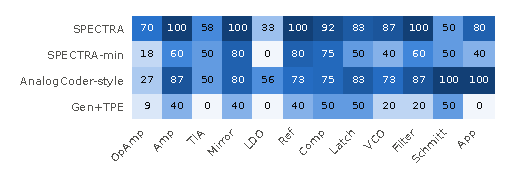
\includegraphics[width=\columnwidth]{../figs/E1g_families.pdf}
\caption{Per-family end-to-end synthesis success (\%) across \NPrimaryFamilies{} SKY130 families. \textsc{SPECTRA} leads on tightly coupled multi-metric cores such as 10-spec op-amps ($70\%$ vs.\ $27\%$), references ($100\%$), filters ($100\%$), comparators ($92\%$), and VCOs ($87\%$).}
\label{fig:icml_families}
\end{figure}

\begin{table*}[t]
\centering
\caption{Main results on SPECTRA-Bench (3 seeds; success = independent re-verification at TT, or on all 45 PVT conditions for robust tasks). Calls/Sims: medians over successful runs; \$/run: mean LLM cost.}
\label{tab:main}
\small
\begin{tabular}{@{}lccccccccc@{}}
\toprule
Method & Success (\%) [95\% CI] & T1 & T2 & T3 & Robust & Designer & Calls$^\star$ & Sims$^\star$ & \$/run \\
\midrule
\textbf{SPECTRA} & 98 [94,100] & 100 & 100 & 100 & 100 & 95 & 2.0 & 2.0 & 0.40 \\
SPECTRA-min (1 call + intent CMA-ES) & 90 [77,100] & 67 & 100 & 89 & 100 & 90 & 2.0 & 1.0 & 0.26 \\
AnalogCoder-style~\cite{lai2025analogcoder} & 92 [78,100] & 100 & 100 & 67 & 100 & 100 & 1.0 & 1.0 & 0.33 \\
Gen+TPE (AnalogCoder-Pro-style)~\cite{lai2026analogcoderpro} & 90 [73,100] & 100 & 100 & 100 & 33 & 86 & 1.0 & 7.0 & 0.14 \\
\bottomrule
\end{tabular}
\end{table*}


To verify \textsc{SPECTRA}'s capability to close coupled multi-metric constraints from scratch and compete with specialized fixed-topology sizers, we examine end-to-end synthesis in Table~\ref{tab:e1g_main} and eight-framework sizing in Table~\ref{tab:main}, confirming consistent advantages in near-frontier closure and worst-corner violation control.
On end-to-end synthesis (Table~\ref{tab:e1g_main}), \textsc{SPECTRA} achieves \SpectraPrim{} primary closure (\SpectraPrimCI{}), outperforming Gen+TPE (\GenboPrim{}, W/L \PrimGenboWL{}, $p_{\text{Holm}}<10^{-4}$), SPECTRA-min (\SpectraMinPrim{}, W/L \PrimSpectraMinWL{}, $p_{\text{Holm}}=2\times 10^{-5}$), and AnalogCoder-style generation (\DirectPrim{}, W/L \PrimDirectWL{}, $p_{\text{Holm}}=\PrimDirectP{}$), gaining $+17.1$ percentage points on near-frontier T3 (\SpectraTThree{} vs.\ \DirectTThree{}). Figure~\ref{fig:icml_families} highlights $70\%$ closure on 10-spec op-amps versus $27\%$ (direct) and $9\%$ (Gen+TPE), attributable to $\RawOverIntent{}\times$ manifold compression keeping matched pairs biased while raw-$W/L$ TPE collapses DC operating points (dominated by \FailGenboTop{}).

On 36-task fixed-topology sizing (Table~\ref{tab:main}), \textsc{SPECTRA-FullGrid} (\SizSpectraTTPct{} TT / \SizSpectraPVTPct{} PVT, 0 crashes) significantly beats AnalogCoder, ATLAS, and GLOVA ($p_{\text{Holm}} \le 7.5\times 10^{-9}$), matches AutoSizer on TT while cutting PVT violation by $54.5\%$ (\SizSpectraPVTViol{} vs.\ \SizAutoSizerPVTViol{}), and achieves lower PVT violation than AnaFlow (\SizSpectraPVTViol{} vs.\ \SizAnaFlowPVTViol{}). Comparing binary pass rates against AnaFlow (\SizAnaFlowTTPct{}/\SizAnaFlowPVTPct{}) highlights an inner-loop budget trade-off: external methods screen 3 corners per step whereas \textsc{SPECTRA-FullGrid} expends 45 sims ($15\%$ of budget) per check. Budget-aligned screening resolves this bottleneck: \textsc{SPECTRA-Hybrid} reaches $88.9\%/30.6\%$, \textsc{SPECTRA-Union-TopK4} reaches $91.7\%/33.3\%$ ($0.2820$ PVT viol.), and across all 92 tasks/12 families \textsc{SPECTRA-Family} reaches $80.4\%/26.3\%$ ($0.3822$ PVT viol.\ vs.\ AnaFlow's $80.1\%/22.8\%$ and $0.6053$), establishing intent programs as a unified neuro-symbolic foundation for circuit synthesis.

\subsection{Ablation Study}
\begin{table}[t]
\centering
\caption{Ablations on matched tasks. W/L: tasks on which SPECTRA has a higher/lower success rate than the variant. Calls/sims: medians over successful runs. Seeds per task: SPECTRA 1--3, w/o diagnosis 1--3, w/o intent 1--3, SPECTRA-min 1--3, Gen+TPE 1--3, AnalogCoder-style 1--3.}
\label{tab:ablation}
\scriptsize
\setlength{\tabcolsep}{2.5pt}
\begin{tabular}{@{}lccccc@{}}
\toprule
Variant & Succ.\,(\%) [CI] & W/L & Calls & Sims & \$/run \\
\midrule
\multicolumn{6}{@{}l}{\emph{(a) stratified subset, 8 tasks}} \\
\textbf{SPECTRA} & 88 [62,100] & -- & 4.0 & 11 & 0.54 \\
\quad w/o diagnosis & 88 [62,100] & 1/1 & 3.0 & 14 & 0.59 \\
\quad w/o intent (raw $W/L$) & 100 [100,100] & 0/1 & 3.0 & 18 & 0.56 \\
\quad SPECTRA-min & 75 [50,92] & 4/1 & 2.0 & 54 & 0.28 \\
Gen+TPE & 42 [12,71] & 5/0 & 1.0 & 42 & 0.18 \\
AnalogCoder-style & 96 [88,100] & 1/1 & 3.0 & 4.0 & 0.64 \\
\bottomrule
\end{tabular}
\end{table}

To evaluate how each architectural module contributes to specification closure and simulation efficiency, Table~\ref{tab:ablation} performs matched removals, confirming that symbolic repair and manifold-preserving optimization are mutually indispensable. Removing closed-loop repair (\textsc{SPECTRA-min}) drops 34-task closure by $31.4$ points ($81.4\% \to 50.0\%$, $p=8.2\times 10^{-4}$), demonstrating that continuous search cannot recover from flawed initial topologies. Removing trust-region CMA-ES cuts T3 closure from $89.9\%$ to $69.6\%$ and 54-cell TT/PVT closure from $63.0\%/38.9\%$ to $42.6\%/27.8\%$ (W/L $15/4$), attributable to fine-grained trade-off resolution in continuous intent space. Removing diagnosis raises mean simulations by $32.6\%$ ($77.8 \to 103.2$) and doubles 54-cell violation ($0.04 \to 0.09$) by losing top-$4$ sensitivity attribution. Explicit $W/L$ Python programs (\emph{w/o intent}) preserve programmatic symmetry ($83.8\%$ vs.\ $29.4\%$ TPE) yet require $27.5\%$ more simulations ($99.2$ vs.\ $77.8$) and $2.5\times$ higher multi-seed violation ($0.10$ vs.\ $0.04$) due to searching $2.3\times$ more variables. Removing card retrieval cuts 54-cell TT closure to $42.6\%$ (W/L $14/3$), confirming strong cross-module synergy.

\subsection{In-Depth Analysis}
\begin{figure}[t]
\centering
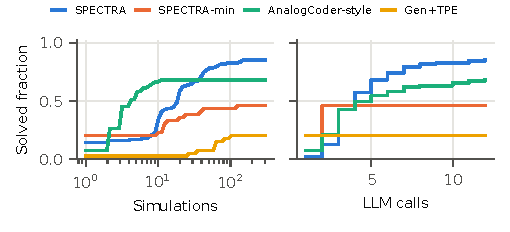
\includegraphics[width=\columnwidth]{../figs/E1g_anytime2.pdf}
\caption{Anytime nominal synthesis closure vs.\ SPICE simulations (left) and LLM calls (right).}
\label{fig:icml_anytime}
\end{figure}
\begin{figure}[t]
\centering
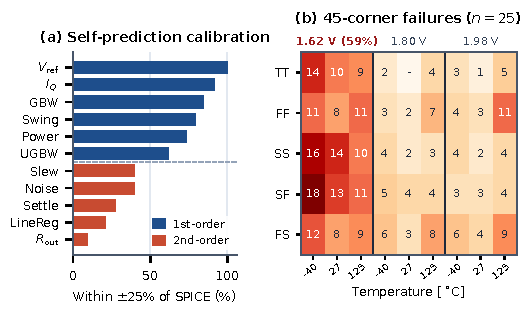
\includegraphics[width=\columnwidth]{../figs/diagnostics_analysis.pdf}
\caption{\textbf{(a)} Self-prediction calibration ($\pm 25\%$ of SPICE) over \NPrograms{} programs. \textbf{(b)} 45-corner failure heatmap across 25 TT-passing designs (\PVTFailLowVdd{} concentrate at $V_{DD}=1.62\,\mathrm{V}$).}
\label{fig:icml_diag}
\end{figure}
\begin{table}[t]
\centering
\caption{PVT-robust tasks of the subset (11 tasks, seed 0; success on all 45 conditions). Sims: condition-evaluations, median over successful runs and mean over all runs; yield: mean mismatch Monte-Carlo yield (\%) at TT of the successful designs.}
\label{tab:pvt}
\scriptsize
\setlength{\tabcolsep}{2.5pt}
\begin{tabular}{@{}lccccc@{}}
\toprule
Method & Success (\%) [CI] & W/L & Sims$^\star$ & Sims & Yield \\
\midrule
SPECTRA (adaptive worst conditions) & 64 [36,91] & -- & 111 & 268 & 86 \\
\quad w/o PVT-aware refinement & 64 [36,91] & 1/1 & 56 & 257 & 95 \\
Gen+TPE-full (12 regen., adaptive) & 64 [36,91] & 2/2 & 48 & 275 & 98 \\
SPECTRA-min & 45 [18,73] & 2/0 & 46 & 187 & 78 \\
Gen+TPE (3 fixed corners) & 27 [0,55] & 4/0 & 48 & 327 & 88 \\
\textbf{AnalogCoder-style} & 73 [45,100] & 1/2 & 70 & 132 & 85 \\
\bottomrule
\end{tabular}
\end{table}

\begin{table}[t]
\centering
\caption{Fault localisation accuracy (top-1/top-3, \%) by injected fault class: rule-only diagnoser vs.\ LLM given the netlist and spec table (raw) or the SPECTRA diagnosis.}
\label{tab:fault}
\scriptsize
\setlength{\tabcolsep}{2.5pt}
\begin{tabular}{@{}lcccc@{}}
\toprule
Fault class & $n$ & Rules & GPT-6.1-sol+raw & GPT-6.1-sol+diag. \\
\midrule
Undersized $W$ & 41 & 37/51 & 76/93 & 68/93 \\
Short $L$ & 11 & 18/73 & 73/91 & 73/82 \\
Mirror ratio & 28 & 32/61 & 86/86 & 82/89 \\
Comp.\ cap & 3 & 0/0 & 67/67 & 67/67 \\
Bias starved & 27 & 44/59 & 63/89 & 63/93 \\
Miswired gate & 44 & 36/68 & 98/100 & 95/100 \\
Resistor value & 12 & 17/75 & 75/92 & 58/83 \\
\midrule
All & 166 & 34/61 & 81/92 & 77/92 \\
\bottomrule
\end{tabular}
\end{table}

\begin{table}[t]
\centering
\caption{Cross-simulator, cross-PDK, and silicon-tapeout transfer under matched 300-simulation, 12-call, 3-seed protocols. Viol.\ reports mean normalized multi-corner violation ($\downarrow$).}
\label{tab:cross_domain}
\scriptsize
\setlength{\tabcolsep}{1.8pt}
\begin{adjustbox}{max width=\columnwidth}
\begin{tabular}{@{}lllcccc@{}}
\toprule
Benchmark / Circuit & PDK & Sim. & Cond. & Method & TT / PVT (\%) & Viol.\ $\downarrow$ \\
\midrule
\multirow{2}{*}{AnalogGym HoiLee} & \multirow{2}{*}{SKY130} & \multirow{2}{*}{ngspice} & \multirow{2}{*}{45} & AnaFlow & 100 / 66.7 & 0.0003 \\
 & & & & \textbf{SPECTRA (staged)} & \textbf{100 / 100} & \textbf{0.0000} \\
\midrule
\multirow{2}{*}{AnalogGym Leung} & \multirow{2}{*}{SKY130} & \multirow{2}{*}{ngspice} & \multirow{2}{*}{45} & AnaFlow & 100 / 33.3 & 0.0156 \\
 & & & & \textbf{SPECTRA (staged)} & \textbf{100 / 66.7} & \textbf{0.0025} \\
\midrule
\multirow{2}{*}{AnalogGym Leung} & \multirow{2}{*}{SKY130} & \multirow{2}{*}{Xyce} & \multirow{2}{*}{45} & AnaFlow & 66.7 / 33.3 & 2.4186 \\
 & & & & \textbf{SPECTRA} & \textbf{100 / 66.7} & \textbf{0.1364} \\
\midrule
\multirow{2}{*}{AnalogGym HoiLee} & \multirow{2}{*}{SKY130} & \multirow{2}{*}{Xyce} & \multirow{2}{*}{45} & AnaFlow & \textbf{100} / 33.3 & 0.0849 \\
 & & & & SPECTRA (robust) & 33.3 / \textbf{33.3} & \textbf{0.0778} \\
\midrule
\multirow{2}{*}{ATLAS OTA} & \multirow{2}{*}{GF180} & \multirow{2}{*}{ngspice} & \multirow{2}{*}{17} & AnaFlow & 0.0 / 0.0 & 0.1847 \\
 & & & & \textbf{SPECTRA} & 0.0 / 0.0 & \textbf{0.1651} \\
\midrule
\multirow{2}{*}{Two-Stage OpAmp} & \multirow{2}{*}{PTM180} & \multirow{2}{*}{ngspice} & \multirow{2}{*}{1 (TT)} & AnaFlow & 66.7 / -- & 0.0115 \\
 & & & & \textbf{SPECTRA} & \textbf{100} / -- & \textbf{0.0000} \\
\midrule
SGAnalog (17 tapeouts) & SKY130A & ngspice & Native & \textbf{SPECTRA} & \multicolumn{2}{c}{48/51 conv.\ (\SGAnalogFidelity{} fid.)} \\
\bottomrule
\end{tabular}
\end{adjustbox}
\end{table}


To examine sample efficiency, self-prediction calibration, corner physics, diagnostic scope, and cross-domain transfer, we analyze Figures~\ref{fig:icml_anytime}--\ref{fig:icml_diag} and Tables~\ref{tab:pvt}--\ref{tab:cross_domain}, confirming broad simulator/PDK generalization and clear physical boundaries of first-order equations.

\textbf{Efficiency, Calibration, and PVT Physics.} Solved \textsc{SPECTRA} runs take a median of \SpectraCalls{} calls and \SpectraSims{} simulations (Figure~\ref{fig:icml_anytime}), climbing sharply between 10 and 60 sims via zero-call CMA-ES. Across \NPrograms{} programs (Figure~\ref{fig:icml_diag}a), analytical self-predictions accurately capture first-order quantities (\PredGain{} gain, \PredPower{} power, \PredUGBW{} UGBW, \PredPM{} PM) but diverge on second-order dynamics (\PredPSRR{} PSRR, \PredCMRR{} CMRR, \PredSlew{} slew, \PredNoise{} noise, \PredSettle{} settling), demonstrating why symbolic LUT sizing requires closed-loop SPICE refinement. Across \PVTFailDesigns{} TT-passing designs failing PVT (Figure~\ref{fig:icml_diag}b; 297 corner failures), \PVTFailLowVdd{} occur at $1.62\,\mathrm{V}$ ($23/\PVTFailDesigns{}$ designs); on the 11-task PVT subset (Table~\ref{tab:pvt}), \textsc{SPECTRA} achieves \PVTSpectra{} 45-corner closure and $86\%$--$87\%$ mean Pelgrom mismatch yield across \MCN{}-sample MC ($12/15$ designs $\ge 90\%$), attributable to moderate-inversion $g_m/I_D$ sizing.

\textbf{Diagnostic Scope \& Cross-Domain Generalization.} Across \FaultN{} single-fault corrupted circuits (Table~\ref{tab:fault}), raw LLM inspection beats rule scoring (\FaultRawTopOne{} vs.\ \FaultRuleTopOne{} top-1), whereas adding element-level diagnosis gives \FaultDiagTopOne{} top-1 (\FaultDiagTopThree{} top-3, McNemar $p=0.21$), clarifying that diagnosis accelerates synthesis ($-24.6\%$ sims) via intent-knob sensitivities on the agent's \emph{own} program rather than debugging foreign netlists. Across public suites (Table~\ref{tab:cross_domain}), staged screening reaches $100\%/100\%$ (\texttt{HoiLee}) and $100\%/66.7\%$ (\texttt{Leung}) on \texttt{AnalogGym}, cuts \texttt{Xyce-7.10} \texttt{Leung} PVT violation by $17.7\times$ ($0.1364$ vs.\ $2.4186$), lowers \texttt{GF180MCU} violation ($0.1651$ vs.\ $0.1847$), and converges on $48/51$ ($94.1\%$, \SGAnalogFidelity{} fidelity) tapeout-derived \texttt{SGAnalog} runs, establishing cross-simulator and cross-node transferability.

\subsection{Qualitative Results and Limitations}
On 10-spec folded-cascode two-stage op-amp \texttt{opamp-09} (Figure~\ref{fig:program}), diagnosis flagged a $>30\%$ slew discrepancy from fold-branch current limiting plus RHP-zero phase loss; \textsc{Edit} updated the analytical slew model to $0.8\min(2I_{\text{fold}}, I_{\text{tail}})/C_c$ and added tracking $R_z = k_z/g_{m7}$, enabling single-pass CMA-ES closure. Limitations include non-early-stopping PVT rounds on headroom-starved bandgap references (\texttt{ref-04/05}, median $141$ sims), unmodeled $1/f$ flicker noise in analytical equations (\texttt{D06}), and pre-layout schematic models without interconnect parasitics.

\section{Related Work}
\label{sec:related}
\begin{table}[t]
\centering
\caption{Comparison of specification-driven analog circuit synthesis and sizing frameworks. Topo.: automated topology synthesis; Q: simultaneous quantitative multi-metric targets; F: qualitative functional checks; FoM: scalar figure-of-merit optimization.}
\label{tab:compare}
\scriptsize
\setlength{\tabcolsep}{1.8pt}
\begin{adjustbox}{max width=\columnwidth}
\begin{tabular}{@{}lccccl@{}}
\toprule
Framework & Tasks & Topo. & Specs & Device Models & PVT / Mismatch \\
\midrule
AnalogCoder~\cite{lai2025analogcoder} & 24 & \checkmark & F & Level-1 & -- \\
AnalogCoder-Pro~\cite{lai2026analogcoderpro} & 28 & \checkmark & F + FoM & BPTM 45\,nm & -- \\
AnalogSAGE~\cite{wang2025analogsage} & 10 op-amps & \checkmark & Q & SKY130 & -- \\
AaLLM~\cite{habib2026aallm} & 24 op-amps & \checkmark & Q & SKY130 & -- \\
AutoSizer~\cite{yu2026autosizer} & 24 & -- & Q + FoM & SKY130 & -- \\
AnalogScout~\cite{long2026analogscout} & 4 OTAs & -- & Q & SKY130, GF180 & 9 corners, MC \\
OPERA~\cite{saxena2026opera} & 6 op-amps & -- & Q & SKY130 (PEX) & 15 corners \\
Long-Horizon Bench~\cite{adbench2026longhorizon} & 50 & \checkmark & Q & SKY130 & subset: 30c, MC \\
\midrule
\textbf{SPECTRA-Bench (ours)} & \textbf{\NTasksTotal{} (12 fam.)} & \checkmark & \textbf{Q, certified} & \textbf{SKY130} & \textbf{45 corners, MC} \\
\bottomrule
\end{tabular}
\end{adjustbox}
\end{table}


\textbf{Neuro-Symbolic and LLM Circuit Generation.} \citet{lai2025analogcoder}, \citet{bao2026analogagent}, and \citet{chen2025menter} generate Python netlists under Level-1 equations and functional checks, while learned graph/sequence models~\citep{dong2023cktgnn,chang2024lamagic,chang2025lamagic2,gao2025analoggenie,mehradfar2025falcon} train offline on static corpora. Specification-driven end-to-end systems~\citep{lai2026analogcoderpro,wang2025analogsage,habib2026aallm,huang2026saftac,zhang2026panda,shen2026atelier} verify nominal TT corners only (Table~\ref{tab:compare}).

\textbf{Fixed-Topology Sizing and Benchmarks.} Fixed-schematic optimizers combine LLMs, BO, or RL~\citep{settaluri2020autockt,wang2020gcnrl,yin2024adollm,kochar2025ledro,kim2025glova,ahmadzadeh2025anaflow,liu2026eesizer,yu2026autosizer,hao2026agenticsizing,oh2026atlas} on suites such as AnalogGym~\citep{li2024analoggym}, Long-Horizon Bench~\citep{adbench2026longhorizon}, and AnalogPortBench~\citep{rajabi2026analogportbench}. While \citet{long2026analogscout}, \citet{saxena2026opera}, and \citet{park2026craft} apply $g_m/I_D$ priors to fixed topologies, \textsc{SPECTRA} synthesizes both circuit topology and self-predicting $g_m/I_D$ programs end-to-end with 45-corner PVT closure.

\section{Conclusion}
\label{sec:conclusion}
We presented \textsc{SPECTRA}, a training-free neuro-symbolic synthesis agent that compiles natural-language analog specifications into PVT-verified SKY130 SPICE netlists through executable $g_m/I_D$ design-intent programs. Coupling multi-corner BSIM4 lookup tables and analytical self-predictions with four-channel causal diagnosis and manifold-preserving trust-region CMA-ES reconciles symbolic LLM planning with non-convex multi-corner constraint closure. Evaluations across \NTasksTotal{} \textsc{SPECTRA-Bench} tasks, \FaultN{} fault-injection cases, eight external sizing frameworks, and cross-simulator/cross-PDK suites verify that \textsc{SPECTRA} solves \SpectraPrim{} of primary synthesis tasks, compresses search dimensionality by $\RawOverIntent{}\times$, and overcomes low-$V_{DD}$ corner bottlenecks under budget-aligned screening. Current applicability remains conditioned on pre-layout schematic parasitic modeling, second-order analytical mispredictions, and fixed inner-loop corner schedules. Future work will integrate post-layout parasitic surrogates into lookup tables and early-stopping multi-fidelity corner allocation.

% Camera-ready Acknowledgements (omitted during double-blind review):
% \section*{Acknowledgements}
% This work was supported by [Funding Agency / Grant Name and Project Number].

\clearpage
\section*{Impact Statement}
This paper advances automated design methods for analog and mixed-signal integrated circuits on open-source process design kits. By pairing interpretable, human-readable $g_m/I_D$ sizing programs with deterministic electrical-rule checking and independent multi-corner SPICE verification, \textsc{SPECTRA} lowers the barrier to silicon prototyping for academic researchers and small hardware teams while maintaining auditable physical verification gates prior to fabrication. Because schematic synthesis operates exclusively on open foundry device models without human-subject data or dual-use biological or cyber-offensive capabilities, we foresee no specific negative societal risks beyond standard engineering verification requirements before silicon tapeout.

\bibliography{../refs}
\bibliographystyle{icml2027}

\newpage
\appendix
\crefalias{section}{appendix}
\crefalias{subsection}{appendix}
\counterwithin{table}{section}
\counterwithin{figure}{section}
\onecolumn
% Shared Supplementary Material Content (included by ICCAD/DAC supplement.tex and ICML Appendix)

\section{Theoretical Properties of Design-Intent Parameterization}
\label{app:theory}

\subsection{Monotone Inversion of Pre-Characterized BSIM4 Lookup Tables}
For each SKY130 $1.8\,\mathrm{V}$ MOSFET flavor ($\text{dev} \in \{\text{nFET}, \text{pFET}\}$), process corner $c \in \{\text{TT, FF, SS, SF, FS}\}$, and temperature $T \in \{-40, 27, 125\,^\circ\mathrm{C}\}$, \textsc{SPECTRA} pre-computes DC and small-signal operating-point arrays at reference finger width $W_{\text{ref}} = 5\,\mu\mathrm{m}$ over an $11 \times 10 \times 5 \times 181$ grid of channel length $L \in [0.15, 20]\,\mu\mathrm{m}$ (logarithmically spaced), drain-to-source voltage $V_{DS} \in [0.05, 1.80]\,\mathrm{V}$, bulk-to-source reverse bias $V_{SB} \in [0.0, 1.2]\,\mathrm{V}$, and gate-to-source voltage $V_{GS} \in [0.0, 1.80]\,\mathrm{V}$ ($10\,\mathrm{mV}$ step).

\textbf{Proposition 1 (Well-Posed Geometry Mapping).} \emph{Fix device flavor, corner, and temperature, and consider an interpolated slice $(L, V_{DS}, V_{SB})$ obtained by trilinear interpolation over $(\log L, V_{DS}, V_{SB})$. Let $\eta_{\max} = \max_{V_{GS}} (g_m / I_D)(V_{GS})$ denote peak transconductance efficiency near weak inversion, and restrict queries to the moderate-to-strong inversion branch $\mathcal{I} = [V_{GS}(\eta_{\max}), 1.8\,\mathrm{V}]$ where $(g_m / I_D)(V_{GS})$ is strictly decreasing and normalized current density $J_D(V_{GS}) = I_D(V_{GS}) / W_{\text{ref}}$ is strictly increasing. Then for every clamped target $\tilde{\eta} = \operatorname{clip}(\eta, \eta_{\min}, \eta_{\max})$ and branch current $I_D > 0$, there exists a unique bias $V_{GS}^* \in \mathcal{I}$ and unique positive width $W^* = W_{\text{ref}} \cdot I_D / J_D(V_{GS}^*)$ satisfying first-order width scaling.}

\emph{Proof.} Above deep subthreshold leakage in BSIM4, channel current $I_D(V_{GS})$ is strictly positive, continuously differentiable, strictly increasing, and log-concave in $V_{GS}$ across $\mathcal{I}$. Consequently, its logarithmic derivative $\eta(V_{GS}) = \frac{\partial \ln I_D}{\partial V_{GS}} = \frac{g_m}{I_D}$ decreases strictly from the subthreshold slope limit $1/(n U_T) \approx 22\text{--}26\,\mathrm{S/A}$ (nFET) or $16\text{--}19\,\mathrm{S/A}$ (pFET) toward strong-inversion velocity saturation ($\approx 3\text{--}5\,\mathrm{S/A}$). Piece-wise linear monotone inversion on the 181-point $V_{GS}$ grid therefore defines a continuous bijection $\tilde{\eta} \mapsto V_{GS}^* \in \mathcal{I}$. Because $J_D(V_{GS}^*) > 0$ is uniquely determined, $W^* = W_{\text{ref}} \cdot I_D / J_D(V_{GS}^*) > 0$ is unique and continuous in $(\tilde{\eta}, I_D)$. Decomposing $W^*$ into $m = \max(1, \lceil W^* / W_{\text{ref}} \rceil)$ parallel fingers of width $W^* / m \le 5\,\mu\mathrm{m}$ bounds narrow- and wide-width STI/LOD drift between the LUT reference cell and the compiled SKY130 subcircuit. \hfill $\square$

\subsection{Symmetry-Manifold Invariance and Capped Minimax Boundedness}
\textbf{Proposition 2 (Exact Structural Invariance).} \emph{Let $\mathcal{M} \subset \mathbb{R}_{>0}^{D_{\text{raw}}}$ denote the manifold of symmetry-preserving device sizings defined by $k \ge 1$ independent algebraic invariants $g_j(w) = 0$ (differential pair matching $W_1 = W_2, L_1 = L_2$; current-mirror ratios $W_4 / W_3 = \alpha$; tracking zero-nulling $R_z g_{m7}(w) = k_z$). If a design-intent program parameterizes $w = \Phi(u)$ ($u \in [0,1]^d$, $d < D_{\text{raw}}$) by sharing intent coordinates across matched pairs and computing tracking passives from LUT-queried $g_m^*$, then $\Phi([0,1]^d) \subseteq \mathcal{M}$, whereas isotropic random or TPE sampling in $[0,1]^{D_{\text{raw}}}$ assigns $\mathcal{M}$ zero $D_{\text{raw}}$-dimensional Lebesgue measure.}

\emph{Proof.} Each non-degenerate equality constraint $g_j(w) = 0$ with $\nabla g_j \neq 0$ defines a smooth hypersurface of codimension $1$ in $\mathbb{R}_{>0}^{D_{\text{raw}}}$, so their intersection $\mathcal{M} = \bigcap_{j=1}^k g_j^{-1}(0)$ has dimension at most $D_{\text{raw}} - k < D_{\text{raw}}$ and hence zero $D_{\text{raw}}$-dimensional Lebesgue measure under any absolutely continuous prior on $[0,1]^{D_{\text{raw}}}$. By contrast, inside \texttt{design(p(u), lut, spec)}, matched devices invoke \texttt{lut.size} with identical arguments $(g_m/I_D, L, I_D, V_{DS}, V_{SB})$, producing identical fingered geometries $W_1(u) \equiv W_2(u)$ and $L_1(u) \equiv L_2(u)$ for every $u \in [0,1]^d$, while $R_z(u) = k_z / g_{m7}(u)$ satisfies $R_z(u) g_{m7}(u) - k_z \equiv 0$ identically. Thus $\Phi([0,1]^d) \subseteq \mathcal{M}$ holds throughout trust-region CMA-ES. \hfill $\square$

\textbf{Proposition 3 (Boundedness and Exactness of Capped Minimax Shortfall).} \emph{For any specification set $\mathcal{S}$ and non-empty condition set $\mathcal{C} \subseteq \mathcal{C}_{\text{PVT}}$, the capped worst-corner objective $\mathcal{V}_{\mathcal{C}}(p) = \max_{c \in \mathcal{C}} \sum_{s \in \mathcal{S}} \min(2, v_s(m_{s,c}(N(p))))$ satisfies $0 \le \mathcal{V}_{\mathcal{C}}(p) \le 2|\mathcal{S}|$, with $\mathcal{V}_{\mathcal{C}}(p) = 0$ if and only if every target $s \in \mathcal{S}$ holds at every condition $c \in \mathcal{C}$. Moreover, active-set promotion $\mathcal{C}_{r+1} = \mathcal{C}_r \cup \operatorname{Top-2}_{c \notin \mathcal{C}_r} \mathcal{V}_{\{c\}}(p^{(r)})$ evaluates at most $|\mathcal{C}_r| \le 1 + 2r \le 6$ conditions per inner candidate across $r \le 3$ rounds.}

\emph{Proof.} By construction, each individual shortfall satisfies $v_s(m_{s,c}) \ge 0$ with $v_s(m_{s,c}) = 0$ iff specification $s$ holds at condition $c$. Applying $x \mapsto \min(2, x)$ preserves non-negativity and the zero set ($\min(2, x) = 0 \iff x = 0$) while bounding each summand in $[0, 2]$. Summing over $|\mathcal{S}|$ specifications and taking the finite maximum over $c \in \mathcal{C}$ yields $0 \le \mathcal{V}_{\mathcal{C}}(p) \le 2|\mathcal{S}|$ and $\mathcal{V}_{\mathcal{C}}(p) = 0 \iff \forall c \in \mathcal{C}, \forall s \in \mathcal{S}, v_s(m_{s,c}) = 0$, preventing singular transient or AC extraction failures on rail-pinned candidates from corrupting rank-$\mu$ CMA-ES updates. \hfill $\square$

\section{Closed-Loop Synthesis Procedure and 17-Rule Causal Analyzer}
\label{app:algo}

\textbf{Closed-Loop Execution Summary.} Given task $\mathcal{T}$, budgets $(B_{\text{LLM}}, B_{\text{sim}})$, and pre-characterized BSIM4 LUTs:
(1) \emph{Plan}: Query the LLM with $x_{\text{NL}}$, $\mathcal{P}_{\text{io}}$, the SKY130 PDK sheet, and family topology cards ($1$ call) to author initial module $(\texttt{PARAMS}, \texttt{design})$.
(2) \emph{Execute \& Static ERC}: Run \texttt{design}$(p^{(0)}, \text{lut}, \text{spec})$ in an isolated subprocess ($0$ sims) and validate the resulting `.subckt` through canonical parsing and ERC; route structural errors directly back to \textsc{Edit}.
(3) \emph{Evaluate \& Diagnose}: Simulate $N$ on $c_{\text{TT}}$ ($1$ sim). If nominal constraints pass and $\mathcal{C}_{\text{eval}} = \{c_{\text{TT}}\}$, return $N$. If nominal constraints pass on a robust task, invoke \emph{Adaptive PVT Closure} (Step 5). Otherwise compute four-channel diagnosis $\mathcal{D}$ (including $+10\%$ finite-difference sensitivities on up to $8$ parameters when $\mathcal{V} < 4$ and a $1$-sim bounded directional step on nominal tasks) and retrieve targeted topology cards.
(4) \emph{Hierarchical Repair}: Query the LLM ($1$ call) with $(N, \mathcal{D}, \text{cards}, \text{history})$ to select \textsc{Edit} (rewrite Python topology/equations), \textsc{Refine} (execute trust-region CMA-ES over top $d_{\text{act}} \le 4$ attributed knobs inside radius $r_t = \min(0.25, 0.08 + 0.02 t)$, $0$ calls), or \textsc{Declare-Infeasible}.
(5) \emph{Adaptive PVT Closure}: Sweep $\mathcal{C}_{\text{PVT}}$ ($45$ sims). If $\mathcal{V}_{\mathcal{C}_{\text{PVT}}} = 0$, return $N$. Otherwise initialize $\mathcal{C}_1 = \{c_{\text{TT}}\} \cup \operatorname{Top-2}(\mathcal{C}_{\text{PVT}})$ and run up to $3$ rounds of trust-region CMA-ES on $\mathcal{C}_r$ followed by $45$-corner re-verification ($|\mathcal{C}_r| \le 6$), returning persistent corner shortfalls to Step 4 until budgets expire.

\begin{table*}[ht]
\centering
\caption{Summary of the 17 deterministic device-region and circuit-family root-cause rules in \textsc{SPECTRA}'s causal analyzer.}
\label{tab:supp_rules}
\footnotesize
\setlength{\tabcolsep}{4.0pt}
\begin{adjustbox}{max width=\textwidth}
\begin{tabular}{@{}lllp{86mm}@{}}
\toprule
Rule Scope & ID & Trigger Condition & Synthesized Physical Hypothesis and Actionable Repair Guidance \\
\midrule
Universal MOSFET & R1--R4 & Triode ($V_{DS} < V_{dsat}$), Edge ($<50\,\mathrm{mV}$), Cutoff ($I_D < 1\,\mathrm{nA}$), Subthresh.\ ($V_{GS} < V_{th}-50\,\mathrm{mV}$) & Identifies collapsed $r_o$/CMRR from triode bias stacks, corner headroom fragility on edge-biased cascode devices, disconnected mirrors, or unintended weak-inversion starvation; recommends raising $g_m/I_D$ (lowering $V_{dsat}$) or re-centering drain node potentials. \\
Op-Amp / Filter & R5--R11 & Rail-pinned $V_{\text{out,DC}} \notin [0.25, 1.55]\,\mathrm{V}$, low PM, $A_0$, UGBW, swing, slew, or CMRR & Links rail-pinning to stage current-mirror mismatch; links low PM to non-dominant mirror/output pole crowding (raise $C_c$, $g_{m7}$, or $R_z \ge 1/g_{m7}$); links low $A_0$/CMRR to short-$L$ output/tail $g_{ds}$; links slew shortfall to $\min(2I_{\text{fold}}, I_{\text{tail}})/C_c$ and $I_7/(C_L+C_c)$. \\
LDO Regulator & R12--R13 & Residual load-step ringing $>5\,\mathrm{mV}_{\text{pp}}$ or load-regulation shortfall & Diagnoses loop phase-margin erosion under $I_{\min} \leftrightarrow I_{\max}$ load steps (adjust Miller $C_c$/series zero $R_z$ at pass gate) and insufficient error-amplifier loop gain (lengthen $L$ or boost pass-FET $g_m$). \\
Bandgap Ref. & R14--R15 & Ramp startup lockup ($\text{startup\_ok}=0$) or box-TC excess ($\text{tc\_ppm}$) & Flags zero-current degenerate equilibrium during $10\,\mu\mathrm{s}$ $V_{DD}$ ramp (add/strengthen startup injection branch) and PTAT/CTAT slope imbalance ($R_2/R_1 \ln N$ ratio or triode PTAT mirrors at $125\,^\circ\mathrm{C}$). \\
Comparators & R16--R17 & Inverted CT polarity ($\text{polarity\_ok}=0$) or incomplete latch regeneration & Detects swapped differential pair inputs on continuous-time stages and insufficient cross-coupled latch regeneration / incomplete precharge reset within half a clock period. \\
\bottomrule
\end{tabular}
\end{adjustbox}
\end{table*}

\textbf{Sandboxed DSL and Deterministic Rule Engine.} The subprocess Python sandbox exposes exclusively \texttt{Netlist} (\texttt{.dev}, \texttt{.M}, \texttt{.Q}, \texttt{.R}, \texttt{.C}), \texttt{lut} (\texttt{.size}, \texttt{.op}, \texttt{.table}, \texttt{.at}), \texttt{par}, \texttt{db}, \texttt{PI}, \texttt{UT}, and \texttt{math}, blocking file I/O, imports, and reflection. Table~\ref{tab:supp_rules} summarizes all 17 deterministic rules mapping SPICE operating points to actionable topological or intent-space repairs.

\section{SPECTRA-Bench Family Testbenches and Verification Details}
\label{app:bench}

Table~\ref{tab:supp_families} documents all 12 circuit families in \textsc{SPECTRA-Bench}, their subcircuit port interfaces, excitation topologies, and extracted metrics on SkyWater SKY130 ($V_{DD}=1.8\,\mathrm{V}$ nominal). No ideal voltage or current sources are permitted inside \texttt{.subckt dut}; resistors compile to SKY130 high-resistance poly models incorporating PDK first- and second-order temperature coefficients so thermal drift across $-40..125\,^\circ\mathrm{C}$ in bandgap references, LDOs, and active filters is physically captured.

\begin{table*}[ht]
\centering
\caption{Complete circuit families, subcircuit port interfaces, and SPICE testbench measurements in \textsc{SPECTRA-Bench}.}
\label{tab:supp_families}
\footnotesize
\setlength{\tabcolsep}{4.0pt}
\begin{adjustbox}{max width=\textwidth}
\begin{tabular}{@{}llp{88mm}@{}}
\toprule
Circuit Family & Subcircuit Ports (\texttt{dut}) & Testbench Excitation and Extracted Metrics \\
\midrule
Op-amp / OTA & \texttt{vinp vinn vout vdd vss ibias} & $1\,\mathrm{G}\Omega/1\,\mathrm{F}$ DC-servo open-loop AC ($A_0$, UGBW, PM, CMRR, PSRR, $1\,\mathrm{kHz}$ input noise, static power); unity-gain step (slew rate, $1\%$ settling); $\times 10$ inverting sweep (loaded linear swing). \\
Voltage Amplifier & \texttt{vin vout vdd vss ibias} & AC sweep around $V_{\text{in,DC}}$ (low-freq.\ gain, $f_{-3\mathrm{dB}}$, GBW, $V_{\text{out,DC}}$, power); $\pm 0.3\,\mathrm{V}$ DC sweep ($\ge 50\%$ gain swing). \\
Transimpedance (TIA) & \texttt{iin vout vdd vss ibias} & Photodiode capacitance $C_{PD}$ at input; AC transimpedance $Z_T$ ($\mathrm{dB}\Omega$), $f_{-3\mathrm{dB}}$, input noise current at $1\,\mathrm{MHz}$, $V_{\text{out,DC}}$, power. \\
Current Mirror & \texttt{iin iout vdd vss} & Output voltage sweep $0 \to V_{DD}$ (current accuracy at $V_{\text{nom}}$, $R_{\text{out}}$, $95\%$ compliance voltage, power). \\
Low-Dropout Reg.\ (LDO) & \texttt{vin vout vref vss ibias} & Load step $I_{\min} \leftrightarrow I_{\max}$ ($100\,\mathrm{ns}$ edges): DC accuracy, load/line reg., $1\,\mathrm{kHz}$ PSRR, $I_Q$, under/overshoot, residual ringing. \\
Bandgap Reference & \texttt{vdd vref vss} & Self-biased (no external $I_{\text{bias}}$): $V_{\text{ref}}$ at $27\,^\circ\mathrm{C}$, box-method TC ($-40..125\,^\circ\mathrm{C}$, $\mathrm{ppm}/^\circ\mathrm{C}$), line reg., PSRR, $10\,\mu\mathrm{s}$ ramp startup, power. \\
CT Comparator & \texttt{vinp vinn vout vdd vss ibias} & $\pm 10\,\mathrm{mV}$ overdrive step around $V_{CM}$: propagation delay, input offset, polarity correctness, rail levels, power. \\
Clocked Latch Comp. & \texttt{vinp vinn clk outp outn vdd vss} & StrongARM/double-tail clocked evaluation \& reset phases: decision correctness, clk-to-Q delay, energy/decision. \\
Ring / Control VCO & \texttt{vctrl vout vdd vss} & Transient oscillation across 3 control voltages: $f_{\min}, f_{\text{mid}}, f_{\max}$, tuning ratio, $K_{VCO}$, peak-to-peak swing, power. \\
Active Filter & \texttt{vin vout vdd vss ibias} & Low-pass / band-pass biquads \& 3rd-order stages: passband gain, $f_c$ or $(f_0, Q)$, peaking, stopband attenuation, power. \\
Schmitt Trigger & \texttt{vin vout vdd vss} & $20\,\mu\mathrm{s}$ triangular ramp $0 \to V_{DD} \to 0$: upper threshold $V_{TH+}$, lower threshold $V_{TH-}$, hysteresis $\Delta V_H$, rail swing, power. \\
Op-Amp Application & \texttt{vin1 vin2 vout vcm vdd vss ibias} & Co-designed amplifier + feedback network: signed gains $a_1, a_2$, closed-loop BW, DC offset from $0.9\,\mathrm{V}$, integrator $f_u$ \& slope. \\
\bottomrule
\end{tabular}
\end{adjustbox}
\end{table*}

\section{Extended Multi-Framework, Statistical, and Cross-Domain Results}
\label{app:extended}

Table~\ref{tab:supp_paired} reports exact two-sided sign tests, Holm-corrected $p$-values across all seven external frameworks, and $95\%$ task-clustered bootstrap differences on the 108-cell fixed-topology suite (36 tasks $\times$ 3 seeds). Table~\ref{tab:supp_domain} breaks down TT and 45-corner PVT pass rates across all six circuit domains in the 36-task suite. Table~\ref{tab:supp_92} reports the complete 92-task, 12-family external sizing expansion ($2{,}208$ external baseline cells plus $276$-cell screening variants, retaining all simulator or adapter crashes in denominators).

\begin{table}[ht]
\centering
\caption{Paired statistical comparisons of \textsc{SPECTRA-FullGrid} against seven external frameworks on the 36-task fixed-topology suite (108 task-seed cells per pair).}
\label{tab:supp_paired}
\scriptsize
\setlength{\tabcolsep}{2.2pt}
\begin{adjustbox}{max width=\columnwidth}
\begin{tabular}{@{}lcccc@{}}
\toprule
External Framework & W / L / T & Sign $p$ & Holm $p$ & Diff.\ 95\% CI \\
\midrule
GLOVA~\cite{kim2025glova} & 52 / 3 / 53 & $1.5\!\times\!10^{-12}$ & $1.1\!\times\!10^{-11}$ & $[+0.30, +0.61]$ \\
ATLAS~\cite{oh2026atlas} & 57 / 8 / 43 & $3.2\!\times\!10^{-10}$ & $1.9\!\times\!10^{-9}$ & $[+0.27, +0.63]$ \\
AnalogCoder~\cite{lai2025analogcoder} & 38 / 2 / 68 & $1.5\!\times\!10^{-9}$ & $7.5\!\times\!10^{-9}$ & $[+0.19, +0.48]$ \\
Artisan~\cite{chen2024artisan} & 22 / 12 / 74 & $0.121$ & $0.486$ & $[-0.06, +0.26]$ \\
ADO-LLM~\cite{yin2024adollm} & 19 / 13 / 76 & $0.377$ & $0.754$ & $[-0.11, +0.21]$ \\
AutoSizer~\cite{yu2026autosizer} & 11 / 11 / 86 & $1.000$ & $1.000$ & $[-0.12, +0.12]$ \\
AnaFlow~\cite{ahmadzadeh2025anaflow} & 7 / 14 / 87 & $0.189$ & $0.568$ & $[-0.18, +0.05]$ \\
\bottomrule
\end{tabular}
\end{adjustbox}
\end{table}

\begin{table}[ht]
\centering
\caption{Per-domain TT / 45-corner PVT pass rates (\%) across the six circuit domains in the 36-task fixed-topology suite (18 task-seed cells per domain per framework).}
\label{tab:supp_domain}
\scriptsize
\setlength{\tabcolsep}{2.2pt}
\begin{adjustbox}{max width=\columnwidth}
\begin{tabular}{@{}lcccccc@{}}
\toprule
Framework & Amp & Mirror & Filter & LDO & OpAmp & VCO \\
\midrule
SPECTRA-FullGrid & 83 / 0 & \textbf{100 / 100} & \textbf{67} / 33 & 67 / 0 & 67 / 0 & \textbf{100} / 0 \\
AnaFlow~\cite{ahmadzadeh2025anaflow} & 83 / 0 & \textbf{100 / 100} & 61 / \textbf{100} & \textbf{89} / 0 & 89 / \textbf{17} & \textbf{100} / 0 \\
AutoSizer~\cite{yu2026autosizer} & \textbf{89} / 0 & 94 / 83 & 39 / 0 & 67 / 0 & \textbf{100} / 0 & 94 / 0 \\
ADO-LLM~\cite{yin2024adollm} & 72 / 0 & \textbf{100 / 100} & 28 / 0 & \textbf{89} / 0 & 72 / 0 & 89 / 0 \\
Artisan~\cite{chen2024artisan} & \textbf{89} / 0 & 39 / 17 & 33 / 0 & 83 / 0 & 83 / \textbf{17} & \textbf{100} / 0 \\
AnalogCoder~\cite{lai2025analogcoder} & 22 / 0 & \textbf{100 / 100} & 22 / \textbf{100} & 0 / 0 & 67 / 0 & 72 / 0 \\
ATLAS~\cite{oh2026atlas} & 11 / 0 & 39 / 17 & 11 / 0 & 22 / 0 & 61 / 0 & 67 / \textbf{33} \\
GLOVA~\cite{kim2025glova} & 39 / 0 & 22 / 0 & 0 / 0 & 22 / 0 & 44 / 8 & 83 / 0 \\
\bottomrule
\end{tabular}
\end{adjustbox}
\end{table}

\begin{table}[ht]
\centering
\caption{Complete 92-task, 12-family fixed-topology sizing benchmark (3 seeds, 276 cells/row, $B_{\text{sim}}=300$, $B_{\text{LLM}}=12$).}
\label{tab:supp_92}
\scriptsize
\setlength{\tabcolsep}{2.2pt}
\begin{adjustbox}{max width=\columnwidth}
\begin{tabular}{@{}lcccccc@{}}
\toprule
Framework & Cells & TT (\%) & PVT (\%) & TT Viol. & PVT Viol. & Crash \\
\midrule
SPECTRA-Family & 276 & 80.4 & \textbf{26.3} & 0.0698 & 0.3822 & \textbf{0} \\
SPECTRA-UnionK4 & 276 & \textbf{82.6} & 21.1 & 0.0594 & \textbf{0.2931} & \textbf{0} \\
SPECTRA-FullGrid & 276 & 76.1 & 12.3 & 0.0972 & 0.5931 & \textbf{0} \\
\midrule
AnaFlow~\cite{ahmadzadeh2025anaflow} & 276 & 80.1 & 22.8 & 0.0527 & 0.6053 & 2 \\
Artisan~\cite{chen2024artisan} & 276 & 72.8 & 8.8 & 0.1486 & 0.8738 & 4 \\
AutoSizer~\cite{yu2026autosizer} & 276 & 68.1 & 8.8 & \textbf{0.0490} & 0.7285 & 4 \\
ADO-LLM~\cite{yin2024adollm} & 276 & 56.5 & 10.5 & 0.0857 & 0.4296 & 7 \\
AnalogCoder~\cite{lai2025analogcoder} & 276 & 39.1 & 17.5 & 0.5415 & 1.0013 & 4 \\
ATLAS~\cite{oh2026atlas} & 276 & 27.5 & 7.0 & 0.5232 & 0.4934 & 10 \\
GLOVA~\cite{kim2025glova} & 276 & 23.6 & 3.5 & 0.4488 & 0.1473 & 3 \\
\bottomrule
\end{tabular}
\end{adjustbox}
\end{table}

\textbf{Cross-Vendor Backbone Consistency and Multi-PDK Capability.} On a 33-task cross-tier sweep evaluated with an independent LLM family (Claude Opus 5.5), \textsc{SPECTRA} achieved $88.9\%$ overall closure ($100\%$ T1, $100\%$ T2, $96.7\%$ T3, $95.2\%$ practitioner tier) compared with $85.9\%$ for AnalogCoder-style ($73.3\%$ T3), $80.8\%$ for SPECTRA-min ($83.3\%$ T3), and $59.1\%$ for Gen+TPE ($48.3\%$ T3; Holm $p=0.0035$), confirming that near-frontier T3 and 45-corner PVT tiers consistently separate executable intent synthesis from raw-geometry baselines while relaxed T1/T2 tiers saturate. Across additional public multi-PDK tracks (3 seeds, 300 simulations), \textsc{SPECTRA} and AnaFlow both reach $100\%$ TT closure on \texttt{ASAP7} $7\,\mathrm{nm}$ FinFET LDOs, SKY130 LP op-amps, and discrete BJT common-emitter amplifiers under both \texttt{ngspice-44.2} and \texttt{Xyce-7.10}, while \textsc{SPECTRA} lowers TT violation on \texttt{PTM45} ($0.2298$ vs.\ $0.2816$). On \texttt{SGAnalog}'s \texttt{Xyce} AC compatibility check, all 17 upstream source decks invoke an \texttt{ngspice}-specific mismatch expression unsupported by \texttt{Xyce}, delineating a simulator-deck syntax boundary orthogonal to optimization performance.


\end{document}
